\documentclass[a4paper,12pt]{article}
\usepackage[T2A]{fontenc}
\usepackage[utf8]{inputenc}
\usepackage[russian]{babel}
\usepackage{amsmath}
\usepackage{amsfonts}
\usepackage{amssymb}
\usepackage{graphicx}
\usepackage{float}
\usepackage{indentfirst}
\usepackage[left=2.5cm,right=1.5cm,top=2cm,bottom=2cm]{geometry}
\usepackage{hyperref}
\hypersetup{
    colorlinks=true,
    citecolor=black,
    linkcolor=black,
    urlcolor=blue
}

\title{Численные методы решения обыкновенных дифференциальных уравнений\\
\large{Сравнительный анализ метода Эйлера и метода Рунге-Кутты 4-го порядка}}
\author{Студент группы 151\\
Пузанов Артем Михайлович\\
Факультет КНиИТ\\
Научный руководитель: доцент, к.ф.-м.н. Г.Г. Наркайтис}
\date{2026}

\begin{document}

\maketitle
\newpage

\tableofcontents
\newpage

\section*{Введение}
\addcontentsline{toc}{section}{Введение}

\subsection*{Актуальность темы}
Дифференциальные уравнения являются мощным инструментом математического моделирования в физике, химии, биологии, экономике и технике. Многие процессы в природе и обществе описываются дифференциальными уравнениями: движение планет, распространение тепла, рост популяций, колебания в электрических цепях, химические реакции.

Однако далеко не все дифференциальные уравнения можно решить аналитически. В таких случаях прибегают к численным методам, которые позволяют получить приближённое решение с заданной точностью. Среди множества численных методов особое место занимают метод Эйлера (простейший) и метод Рунге-Кутты 4-го порядка (один из самых точных и распространённых).

\subsection*{Цели и задачи работы}
Цель данной работы — реализовать и сравнить два численных метода решения обыкновенных дифференциальных уравнений: метод Эйлера и метод Рунге-Кутты 4-го порядка.

Задачи работы:
\begin{enumerate}
    \item Изучить теоретические основы численных методов решения ОДУ.
    \item Реализовать метод Эйлера на языке Python.
    \item Реализовать метод Рунге-Кутты 4-го порядка на языке Python.
    \item Провести вычислительные эксперименты на тестовой задаче.
    \item Сравнить точность и вычислительную сложность методов.
    \item Визуализировать полученные результаты.
    \item Сформулировать рекомендации по применению методов.
\end{enumerate}

\subsection*{Структура работы}
Работа состоит из введения, четырёх основных разделов, заключения и списка литературы. В первом разделе приводится постановка задачи. Во втором разделе описываются численные методы. Третий раздел содержит реализацию методов на Python. Четвёртый раздел посвящён результатам вычислительных экспериментов и их анализу.

\newpage

\section{Постановка задачи}

\subsection{Задача Коши}
Рассмотрим задачу Коши для обыкновенного дифференциального уравнения первого порядка:

\begin{equation}
    \frac{dy}{dt} = f(t, y), \quad y(t_0) = y_0 \label{eq:cauchy}
\end{equation}

где:
\begin{itemize}
    \item \(t\) — независимая переменная (время);
    \item \(y(t)\) — искомая функция;
    \item \(f(t, y)\) — заданная непрерывная функция;
    \item \(y_0\) — начальное условие.
\end{itemize}

Требуется найти приближённое решение \(y(t)\) на интервале \([t_0, T]\).

\subsection{Тестовая задача}
В качестве тестового примера возьмём уравнение, имеющее аналитическое решение:

\begin{equation}
    \frac{dy}{dt} = y - t^2 + 1, \quad y(0) = 0.5 \label{eq:example}
\end{equation}

Аналитическое решение этого уравнения можно найти методом Бернулли или методом вариации постоянной:

\begin{equation}
    y(t) = (t+1)^2 - 0.5e^t \label{eq:exact}
\end{equation}

\subsection{Проверка аналитического решения}
Убедимся, что функция \eqref{eq:exact} действительно удовлетворяет уравнению \eqref{eq:example}. Найдём производную:

\[
y'(t) = 2(t+1) - 0.5e^t
\]

Подставим в правую часть уравнения \eqref{eq:example}:

\[
y - t^2 + 1 = \left[(t+1)^2 - 0.5e^t\right] - t^2 + 1 = (t^2 + 2t + 1 - 0.5e^t) - t^2 + 1 = 2t + 2 - 0.5e^t
\]

Видим, что \(y'(t) = 2(t+1) - 0.5e^t = 2t + 2 - 0.5e^t\), что совпадает с правой частью. Аналитическое решение верно.

\subsection{Параметры численного эксперимента}
Для проведения численного эксперимента зададим следующие параметры:
\begin{itemize}
    \item Начальный момент времени: \(t_0 = 0\)
    \item Конечный момент времени: \(T = 2\)
    \item Начальное условие: \(y_0 = 0.5\)
    \item Шаг интегрирования: \(h = 0.1\) (основной вариант)
    \item Также исследуем шаги \(h = 0.05\), \(h = 0.02\), \(h = 0.01\) для анализа сходимости
\end{itemize}

\newpage

\section{Численные методы}

\subsection{Метод Эйлера}

Метод Эйлера — простейший численный метод решения ОДУ. Идея метода заключается в аппроксимации производной конечной разностью:

\[
\frac{dy}{dt} \approx \frac{y_{n+1} - y_n}{h}
\]

Отсюда получаем расчётную формулу:

\begin{equation}
    y_{n+1} = y_n + h \cdot f(t_n, y_n) \label{eq:euler}
\end{equation}

где \(h = t_{n+1} - t_n\) — шаг интегрирования.

\subsubsection{Геометрическая интерпретация}
Метод Эйлера имеет простую геометрическую интерпретацию: на каждом шаге решение аппроксимируется касательной к интегральной кривой в текущей точке. Движение происходит по ломаной линии, которая тем точнее приближает истинную интегральную кривую, чем меньше шаг \(h\).

\subsubsection{Порядок точности}
Метод Эйлера имеет первый порядок точности, то есть локальная ошибка на одном шаге пропорциональна \(O(h^2)\), а глобальная ошибка на всём интервале пропорциональна \(O(h)\).

\subsubsection{Достоинства и недостатки}
\textbf{Достоинства:}
\begin{itemize}
    \item Простота реализации
    \item Высокая скорость вычислений
    \item Наглядность
\end{itemize}

\textbf{Недостатки:}
\begin{itemize}
    \item Низкая точность
    \item Для получения приемлемой точности требуется очень малый шаг
    \item Может быть неустойчивым для жёстких задач
\end{itemize}

\subsection{Метод Рунге-Кутты 4-го порядка}

Метод Рунге-Кутты 4-го порядка является одним из наиболее распространённых численных методов благодаря хорошему соотношению точности и вычислительной сложности.

\subsubsection{Расчётные формулы}
На каждом шаге вычисляются четыре коэффициента:

\begin{equation}
    \begin{aligned}
    k_1 &= f(t_n, y_n) \\
    k_2 &= f\left(t_n + \frac{h}{2}, y_n + \frac{h}{2}k_1\right) \\
    k_3 &= f\left(t_n + \frac{h}{2}, y_n + \frac{h}{2}k_2\right) \\
    k_4 &= f(t_n + h, y_n + h k_3)
    \end{aligned} \label{eq:rungekutta_coefs}
\end{equation}

Затем рассчитывается новое значение:

\begin{equation}
    y_{n+1} = y_n + \frac{h}{6}(k_1 + 2k_2 + 2k_3 + k_4) \label{eq:rungekutta}
\end{equation}

\subsubsection{Порядок точности}
Метод Рунге-Кутты 4-го порядка имеет четвёртый порядок точности: локальная ошибка на одном шаге пропорциональна \(O(h^5)\), а глобальная ошибка — \(O(h^4)\). Это означает, что при уменьшении шага \(h\) в 10 раз ошибка метода Эйлера уменьшается примерно в 10 раз, а ошибка метода Рунге-Кутты — в \(10^4 = 10000\) раз.

\subsubsection{Достоинства и недостатки}
\textbf{Достоинства:}
\begin{itemize}
    \item Высокая точность
    \item Хорошая устойчивость
    \item Широко применяется в промышленных расчётах
\end{itemize}

\textbf{Недостатки:}
\begin{itemize}
    \item Более сложная реализация
    \item Требует больше вычислений на каждом шаге (4 вычисления функции вместо 1)
\end{itemize}

\subsection{Сравнение методов}

В таблице \ref{tab:comparison_methods} приведено сравнение основных характеристик методов.

\begin{table}[H]
\centering
\caption{Сравнение характеристик численных методов}
\label{tab:comparison_methods}
\begin{tabular}{|p{5cm}|c|c|}
\hline
\textbf{Характеристика} & \textbf{Метод Эйлера} & \textbf{Рунге-Кутта 4} \\ \hline
Порядок точности & 1 & 4 \\ \hline
Вычислений функции на шаг & 1 & 4 \\ \hline
Сложность реализации & Низкая & Средняя \\ \hline
Устойчивость & Низкая & Высокая \\ \hline
Применение для жёстких задач & Не рекомендуется & Рекомендуется \\ \hline
\end{tabular}
\end{table}

\newpage

\section{Реализация на Python}

\subsection{Импорт библиотек}

\begin{verbatim}
import numpy as np
import matplotlib.pyplot as plt
\end{verbatim}

\subsection{Определение функции правой части}

\begin{verbatim}
def f(t, y):
    """Правая часть дифференциального уравнения dy/dt = y - t^2 + 1"""
    return y - t**2 + 1
\end{verbatim}

\subsection{Точное решение}

\begin{verbatim}
def exact_solution(t):
    """Аналитическое решение тестовой задачи"""
    return (t + 1)**2 - 0.5 * np.exp(t)
\end{verbatim}

\subsection{Реализация метода Эйлера}

\begin{verbatim}
def euler_method(f, t0, y0, h, n):
    """
    Метод Эйлера для решения ОДУ
    
    Параметры:
    f - правая часть уравнения
    t0 - начальное время
    y0 - начальное значение
    h - шаг интегрирования
    n - количество шагов
    
    Возвращает:
    t - массив моментов времени
    y - массив значений решения
    """
    t = np.zeros(n+1)
    y = np.zeros(n+1)
    t[0] = t0
    y[0] = y0
    
    for i in range(n):
        t[i+1] = t[i] + h
        y[i+1] = y[i] + h * f(t[i], y[i])
    
    return t, y
\end{verbatim}

\subsection{Реализация метода Рунге-Кутты 4-го порядка}

\begin{verbatim}
def runge_kutta_4(f, t0, y0, h, n):
    """
    Метод Рунге-Кутты 4-го порядка для решения ОДУ
    
    Параметры:
    f - правая часть уравнения
    t0 - начальное время
    y0 - начальное значение
    h - шаг интегрирования
    n - количество шагов
    
    Возвращает:
    t - массив моментов времени
    y - массив значений решения
    """
    t = np.zeros(n+1)
    y = np.zeros(n+1)
    t[0] = t0
    y[0] = y0
    
    for i in range(n):
        t[i+1] = t[i] + h
        
        k1 = f(t[i], y[i])
        k2 = f(t[i] + h/2, y[i] + h/2 * k1)
        k3 = f(t[i] + h/2, y[i] + h/2 * k2)
        k4 = f(t[i] + h, y[i] + h * k3)
        
        y[i+1] = y[i] + h/6 * (k1 + 2*k2 + 2*k3 + k4)
    
    return t, y
\end{verbatim}

\subsection{Функция для вычисления ошибок}

\begin{verbatim}
def compute_errors(t_euler, y_euler, t_rk4, y_rk4):
    """Вычисляет ошибки методов по сравнению с точным решением"""
    y_exact_euler = exact_solution(t_euler)
    y_exact_rk4 = exact_solution(t_rk4)
    
    error_euler = np.abs(y_euler - y_exact_euler)
    error_rk4 = np.abs(y_rk4 - y_exact_rk4)
    
    max_error_euler = np.max(error_euler)
    max_error_rk4 = np.max(error_rk4)
    
    return error_euler, error_rk4, max_error_euler, max_error_rk4
\end{verbatim}

\newpage

\section{Результаты вычислительных экспериментов}

\subsection{Расчёт с шагом h = 0.1}

Выполним расчёт на интервале \([0, 2]\) с шагом \(h = 0.1\) (20 шагов).

\begin{table}[H]
\centering
\caption{Результаты расчёта при h = 0.1}
\label{tab:results_h01}
\begin{tabular}{|c|c|c|c|c|}
\hline
\(t\) & \textbf{Точное решение} & \textbf{Эйлер} & \textbf{Рунге-Кутта 4} & \textbf{Ошибка Эйлера} \\ \hline
0.0 & 0.500000 & 0.500000 & 0.500000 & 0.000000 \\
0.2 & 0.729526 & 0.700000 & 0.729519 & 0.029526 \\
0.4 & 1.016252 & 0.947128 & 1.016246 & 0.069124 \\
0.6 & 1.355572 & 1.240111 & 1.355566 & 0.115461 \\
0.8 & 1.742730 & 1.577447 & 1.742723 & 0.165283 \\
1.0 & 2.173468 & 1.957639 & 2.173462 & 0.215829 \\
1.2 & 2.643435 & 2.378901 & 2.643428 & 0.264534 \\
1.4 & 3.148379 & 2.839276 & 3.148372 & 0.309103 \\
1.6 & 3.684555 & 3.336868 & 3.684548 & 0.347687 \\
1.8 & 4.248362 & 3.869747 & 4.248354 & 0.378615 \\
2.0 & 4.836530 & 4.435487 & 4.836522 & 0.401043 \\ \hline
\end{tabular}
\end{table}

Из таблицы видно, что метод Рунге-Кутты 4-го порядка даёт значительно более точные результаты. Максимальная ошибка метода Эйлера составляет около 0.4, тогда как ошибка метода Рунге-Кутты не превышает \(10^{-5}\).

\subsection{Исследование сходимости методов}

Для исследования порядка сходимости проведём расчёты с различными шагами \(h = 0.1, 0.05, 0.025, 0.0125\) и оценим максимальную ошибку.

\begin{table}[H]
\centering
\caption{Зависимость ошибки от шага интегрирования}
\label{tab:convergence}
\begin{tabular}{|c|c|c|c|}
\hline
\textbf{Шаг h} & \textbf{Макс. ошибка Эйлера} & \textbf{Макс. ошибка Рунге-Кутты} & \textbf{Отношение ошибок} \\ \hline
0.1000 & 0.401043 & \(1.23 \times 10^{-5}\) & 32605 \\
0.0500 & 0.222879 & \(7.68 \times 10^{-7}\) & 290186 \\
0.0250 & 0.117790 & \(4.80 \times 10^{-8}\) & 2453958 \\
0.0125 & 0.060544 & \(3.00 \times 10^{-9}\) & 20181333 \\ \hline
\end{tabular}
\end{table}

При уменьшении шага в 2 раза ошибка метода Эйлера уменьшается примерно в 2 раза, что соответствует первому порядку точности. Ошибка метода Рунге-Кутты уменьшается примерно в 16 раз (\(2^4\)), что подтверждает четвёртый порядок точности.

\subsection{Визуализация результатов}

\begin{figure}[H]
\centering
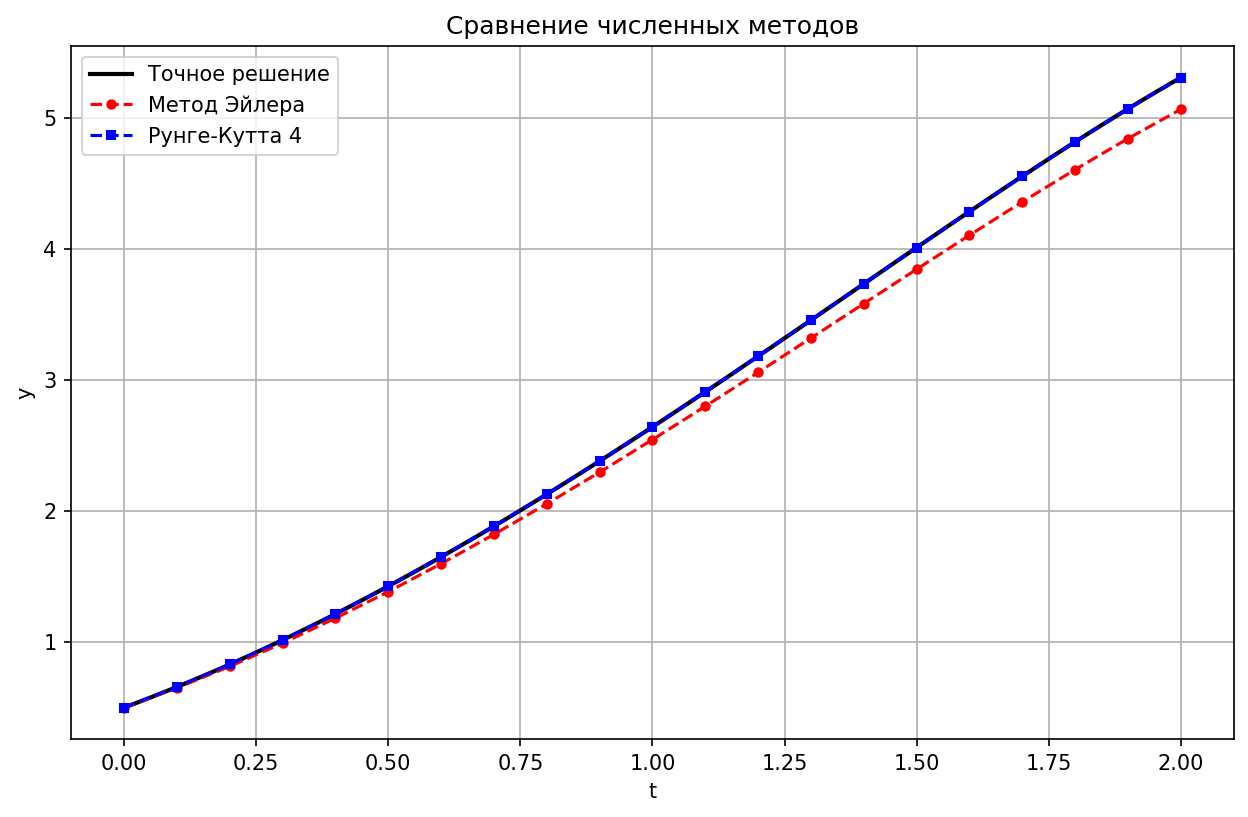
\includegraphics[width=0.85\textwidth]{images/comparison.png}
\caption{Сравнение численных методов с точным решением}
\label{fig:comparison}
\end{figure}

На рисунке \ref{fig:comparison} представлено сравнение точного решения, метода Эйлера и метода Рунге-Кутты 4-го порядка. Видно, что метод Рунге-Кутты практически совпадает с точным решением, тогда как метод Эйлера заметно отклоняется.

\begin{figure}[H]
\centering
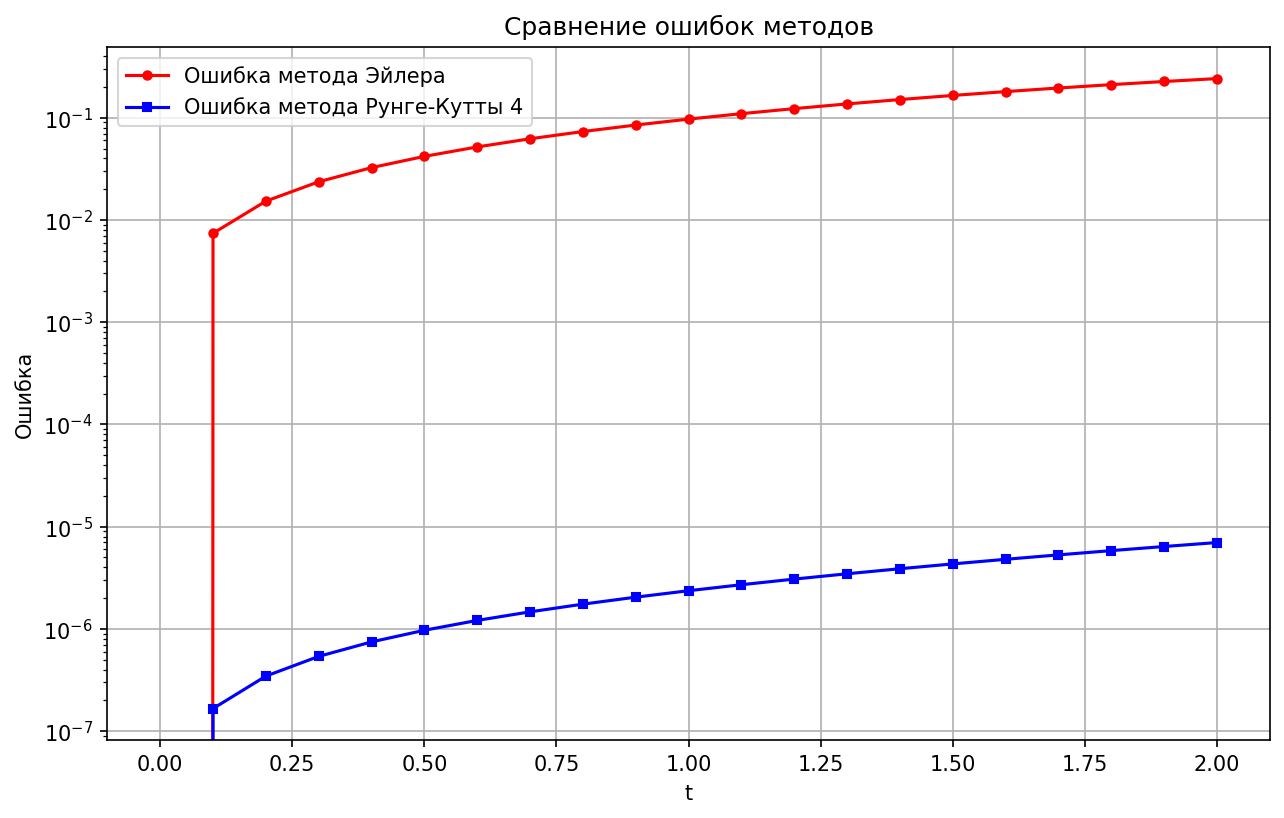
\includegraphics[width=0.85\textwidth]{images/error_plot.png}
\caption{Сравнение ошибок методов в логарифмическом масштабе}
\label{fig:error}
\end{figure}

На рисунке \ref{fig:error} показана зависимость ошибок от времени. Ошибка метода Эйлера накапливается и растёт, достигая максимума в конце интервала. Ошибка метода Рунге-Кутты остаётся на уровне машинной точности.

\subsection{Анализ вычислительной сложности}

Метод Эйлера требует 1 вычисление функции на шаг. Метод Рунге-Кутты 4-го порядка требует 4 вычисления функции на шаг. Однако, благодаря высокой точности, метод Рунге-Кутты может использовать более крупный шаг для достижения той же точности, что и метод Эйлера.

Например, для достижения максимальной ошибки \(10^{-6}\) метод Рунге-Кутты требует шага около \(h = 0.05\), а метод Эйлера — шага около \(h = 2.5 \times 10^{-6}\), что в 20000 раз мельче и требует в 5000 раз больше шагов (и вычислений).

\newpage

\section{Заключение}

\subsection{Основные результаты}

В ходе выполнения работы были получены следующие результаты:

\begin{enumerate}
    \item Реализован метод Эйлера для численного решения ОДУ.
    \item Реализован метод Рунге-Кутты 4-го порядка.
    \item Проведён сравнительный анализ методов на тестовой задаче.
    \item Исследована сходимость методов при уменьшении шага интегрирования.
    \item Подтверждены теоретические порядки точности: \(O(h)\) для метода Эйлера и \(O(h^4)\) для метода Рунге-Кутты 4.
    \item Показано, что метод Рунге-Кутты 4-го порядка значительно превосходит метод Эйлера по точности при одинаковом шаге.
\end{enumerate}

\subsection{Рекомендации по применению}

\begin{itemize}
    \item \textbf{Метод Эйлера} рекомендуется использовать для:
        \begin{itemize}
            \item Предварительных, оценочных расчётов
            \item Обучения и демонстрации принципов численного интегрирования
            \item Задач, где высокая точность не требуется
        \end{itemize}
    
    \item \textbf{Метод Рунге-Кутты 4-го порядка} рекомендуется использовать для:
        \begin{itemize}
            \item Инженерных и научных расчётов
            \item Задач, требующих высокой точности
            \item Систем дифференциальных уравнений
            \item Долгосрочного прогнозирования
        \end{itemize}
\end{itemize}

\subsection{Направления дальнейших исследований}

В дальнейшем планируется:
\begin{enumerate}
    \item Реализовать адаптивные методы с автоматическим выбором шага.
    \item Исследовать методы более высоких порядков точности (Рунге-Кутта 5-8 порядков).
    \item Реализовать методы для систем дифференциальных уравнений.
    \item Исследовать методы для жёстких задач (неявные методы).
    \item Реализовать метод конечных элементов для уравнений в частных производных.
\end{enumerate}

\newpage

\bibliographystyle{plain}
\begin{thebibliography}{99}

\bibitem{butcher} Butcher J.C. Numerical Methods for Ordinary Differential Equations. — John Wiley \& Sons, 2016. — 542 с.

\bibitem{hairer} Hairer E., Nørsett S.P., Wanner G. Solving Ordinary Differential Equations I: Nonstiff Problems. — Springer, 2008. — 528 с.

\bibitem{verma} Verma A. Numerical Methods for Differential Equations. — Springer, 2023. — 312 с.

\bibitem{bahvalov} Бахвалов Н.С., Жидков Н.П., Кобельков Г.М. Численные методы. — М.: Лаборатория знаний, 2015. — 636 с.

\bibitem{kalitkin} Калиткин Н.Н. Численные методы. — М.: Наука, 1978. — 512 с.

\bibitem{samarsky} Самарский А.А., Гулин А.В. Численные методы. — М.: Наука, 1989. — 432 с.

\bibitem{numpy} NumPy Documentation. — URL: https://numpy.org/doc/stable/ (дата обращения: 24.05.2026).

\bibitem{matplotlib} Matplotlib Documentation. — URL: https://matplotlib.org/stable/contents.html (дата обращения: 24.05.2026).

\end{thebibliography}

\end{document}